\section{Results and Conclusion}

\begin{figure}[!htb]
%  \centering
%  \begin{tabular}{|c | c|}
%    \hline
%    Benchmark & P-Value
%    \\ \hline
%    asymptotics & $1.5 \times 10^{-161}$
%    \\ \hline
%    conv\_eval & $9.9 \times 10^{-261}$
%    \\ \hline
%    stlc & $8.2 \times 10^{-309}$
%    \\ \hline
%    stlc5k & $3.6 \times 10^{-305}$
%    \\ \hline
%    stlc10k & DNF
%    \\ \hline
%    stlc100k & DNF
%    \\ \hline
%    stlc\_lessimpl & $4.1 \times 10^{-311}$
%    \\ \hline
%    stlc\_lessimpl5k & $0$
%    \\ \hline
%    stlc\_lessimpl10k & DNF
%    \\ \hline
%    stlc\_small & $0$
%    \\ \hline
%    stlc\_small10k & $2.6 \times 10^{-284}$
%    \\ \hline
%    stlc\_small5k & $1.8 \times 10^{-301}$
%    \\ \hline
%  \end{tabular}
  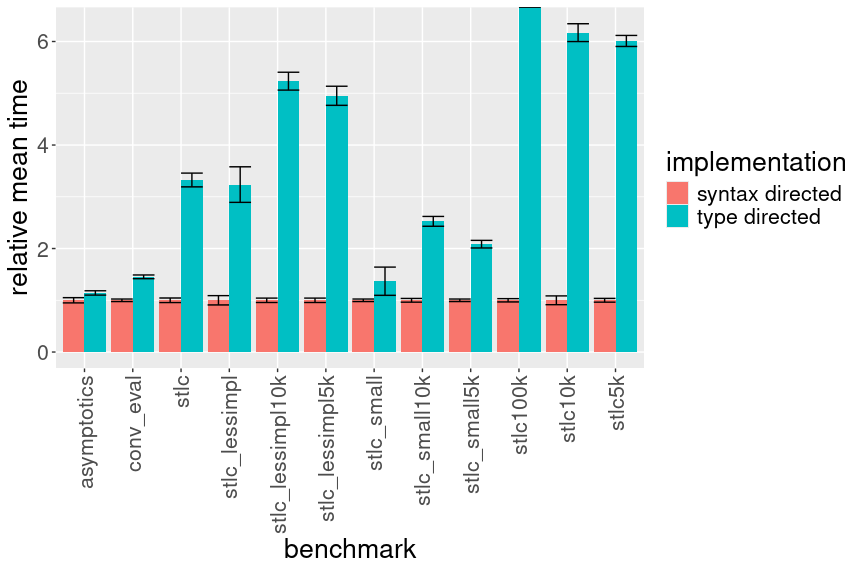
\includegraphics[totalheight=16em]{images/benchmark_graph.png}
  \caption{Benchmark Results}
  \label{fig:results}
\end{figure}

In \autoref{fig:results} we can see the results of the performance comparison between the original syntax-directed smalltt and our modified type-directed smalltt.
Each benchmark was run ten times on an AMD Ryzen 9 3900x processor with 16G of memory.
The results for each benchmark are normalized so that the times for the typed-directed implementation are given as a multiple of the syntax-directed times.

Overall, the type-directed implementation performs worse, being on average 3.4 times slower than the syntax-directed implementation.
In the case of the stlc100k benchmark, the type-directed implementation failed to complete due to running out of memory.
We represent this as a column which continues off the top of the graph to infinity.
\todo{How does this compare to e.g. Rocq or Agda?}

We conjecture that the main reason for this discrepancy is that the syntax-directed implementation is able to take greater advantange of glued evaluation.
Glued evaluation exploits two facts to speed up the judgemental equality check.
Both that substitution and evaluation are functions with respect to judgemental equality, i.e. if $\tyEqJ{\Gamma, x : A}{e}{e'}{B}$ then both $\tyEqJ{\Gamma}{\subst{e}{x}{d}}{\subst{e'}{x}{d}}{B}$ and $\tyEqJ{\Gamma}{v}{v'}{B}$ where $\steps{e}{n}$ and $\steps{e'}{n'}$.
Using this fact, we can avoid normalizing or performing a substitution on terms we are checking for equality if they are already judgementally equal.

Glued evaluation comes to a head when comparing terms whose types contain many redexes.
Since we can only compare terms with the same type for equality, we must first compare the types of the terms, and glued evaluation lets us perform this comparison without computing many of the redexes.
In the type-directed implementation, however, we still fully normalize the type of both terms, since we need to know if it is a type at which we can apply an $\eta$ rule.

This conjecture leads us to the prediction that the performance difference between the syntax and type-directed implementations should correlate with the complexity of types used in the benchmark.
Indeed we find that the benchmark for which the syntax and type-directed implementations are closest is the asymptotics benchmark which contains very little type-level computation, while the difference for the stlc benchmarks, which use quite complicated types to encode the syntax of the simply typed $\lambda$-calculus, is much larger.

As future work, we would like to further investigate this conjecture, and if it proves to be true, investigate if we can improve the performance of the type-directed approach.

There are other procedures for deriving a type-directed algorithm.
For example, in \citet{elabzoo}, the type of each term is calculated during normalization and then stored with the normalized term, so it can be inspected as needed during the equality check.
Although this approach may carry more type information around, if the performance difference is caused by normalizing types and not by allocating types, this could be more performant.

% In \autoref{fig:results} we can see the results of the performance comparison between the original syntax-directed smalltt and our modified type-directed smalltt.
% The p-value is the probability that we got the observed benchmark results under the assumption that our modified version smalltt isn't slower than the original.
% Across the board this probability is very small, and so it seems likely that our modified version of smalltt is slower than the original.
% That being said, a few cases jump out in this table.
% 
% In the stlc\_lessimpl5k and stlc\_small benchmarks, the p-value is 0.
% We interpret this as a p-value so small that it can't be represented as a double-precision floating point number, since these are what we used to do the statistical test.
% 
% Our modified version of smalltt did not finish the stlc10k, stlc100k, and stlc\_lessimpl10k benchmarks due to running out of memory.
% That our implementation failed to complete some of the benchmarks isn't entirely surprising.
% smalltt includes equivalent benchmarks for some other common theorem provers such as Agda, Coq, and Idris2.
% In the performance comparison given in the README for smalltt, both Agda and Idris2 also failed to finish on the stlc100k.
% 
% This, however, doesn't detract from the fact that the original smalltt is clearly faster than our implementation.
% Therefore, we can reject our thesis statement and say that while the type-directed equality supports more rules than the syntax-directed equality, the syntax-directed equality performs better.


